\documentclass[12pt,a4paper,english]{article}
\usepackage[utf8x]{inputenc}
\usepackage{cite}
\usepackage{graphicx}
\usepackage{ucs}
\usepackage{babel}
\usepackage{fancyref}
\usepackage{relsize}
\usepackage{units}
\usepackage{listings}
\usepackage{color}
\usepackage{mathpazo}
\usepackage[
  unicode=true,
  pdftitle={Monte-Carlo Ising Model Simulation of a Two Dimensional Ferromagnet},
  pdfauthor={},
  bookmarks=true,
  bookmarksnumbered=false,
  bookmarksopen=false,
  breaklinks=false,
  pdfborder={0 0 0},
  backref=false,
  colorlinks=false
]{hyperref}

\setlength{\parskip}{1 ex}

\author{}
\title{Monte-Carlo Ising Model Simulation of a Two Dimensional Ferromagnet}
\begin{document}
\maketitle

\begin{abstract}
some text
\end{abstract}

\section{Introduction}
\label{sec:introduction}
In materials the interplay between minimising energy and maximising entropy leads to complex behaviour, including phase transitions where a physical property of a system changes abruptly as thermodynamic variable changes.  Thermodynamic analysis of such problems is only tractable for very simply problems, to which real life situations can be approximated.

The Ising model\cite{brush67} assumes an infinite lattice of points with ``spin'' pointing either up or down (taken as positive or negative for this paper).  The energy $E$ of the lattice is defined by:
\begin{equation}
\label{eq:ising-energy}
E = - \sum_{\mathrm{neighbours}\: i,j} J \sigma_i \sigma_j - \sum_i \mu H \sigma_i
\end{equation}
Where $\sigma_i$ is the spin of the ith lattice point, $J$ is an interaction energy and $\mu H$ is a self-energy.  In the case where $\mu$ is a magnetic moment, $H$ is an external magnetic field and $J$ is a coupling constant the Ising model represents a ferromagnet where each domain interacts only with its nearest neighbours.

The Ising model can be analytically solved in one and two dimensions.  In both when $J>0$ a low temperature phase with spins aligning is seen with a transition to an unordered high temperature phase at the critical temperature $T_c$.  For the case where the model represents a ferromagnet, this low temperature phase is magnetic.  In the case where $J<0$ there is still (anti-aligned order) at low temperature and no order at high temperature.  As both are not magnetic there is no physical property in which to see a phase change.

Onsager \cite{onsager44} showed that in the two dimensional case $\sinh^2 \left(2J/kT_c\right)=1$, i.e.
\begin{equation}
\label{eq:T-c}
T_c= \frac{2} {\ln \left( 1 + \sqrt{2}\right)} \frac{J}{k_B} = 2.269 \frac{J}{k_B}
\end{equation}

Frequently behaviour near phase transitions are approximated by behaviour $\propto \left( T_c - T\right)^\beta$, where $\beta$ is the `critical exponent'. Onsager showed that (as clarified in \cite{montroll63}) the critical exponent is $1/8$:
\begin{eqnarray}
\label{eq:critical-exponent}
M & = & \left( 1- \sinh^{-4} \left(2J/kT \right) \right)^{1/8} \\
  & = & \left( 1- \sinh^{-4} \left[\ln \left(1+\sqrt{2}\right) \frac{T_c}{T} \right] \right)^{1/8} \\
  & \approx & \left( T_c - T \right)^{1/8} \qquad \textrm{around } T=T_c
\end{eqnarray}

As no analytic solution exists in three dimensions, numerical methods for investigating the Ising model are of interest.  One such method is to directly simulate the time evolution of a finite lattice until equilibrium is reached.

\medskip

Further predictions about the system can be made using more general thermodynamic results.  For example we can relate the heat capacity $C$ to the standard deviation of the energy, $\sigma_E$ as it fluctuates with time\cite{rosser82-e-fluc}:

\begin{equation}
\label{eq:e-fluc}
\sigma_E^2=k_B T^2 C
\end{equation}

\section{Method}
\label{sec:method}

This simulation uses a \emph{finite} lattice of spins with periodic boundary conditions as an approximation of the infinite lattice called for by the Ising model.  The simulation progresses by choosing a point on the lattice and calculating the change in energy, defined by \fref[plain]{eq:ising-energy}, that would occur if the spin was flipped.  The Boltzmann probability of the site being in a state with sufficient energy to flip (assuming it is in contact with a resevoir at temperature $T$) $\exp\left(-\Delta E / k_B T\right)$ is calculated.  If this is greater than a random number in the interval [0,1) the lattice point is flipped.

This is continued for sufficient time for equilibrium to reach, when the equilibrium properties of the system can be measured.  We will measure `specific' values of each property, i.e\ per lattice point.  The specific energy, $\epsilon$, is thus the energy calculated by \fref[plain]{eq:ising-energy} divided by the number of lattice points, the specific `magnetisation', $M$, is the absolute value of the mean spin. A estimate of the specific heat capacity, $C_f$, will be made by measuring the size of fluctuation of $epsilon$ using \fref[plain]{eq:e-fluc}.

Simulations will be run across a range of temperatures.  This allows the behaviour of the specific energy and magnetisation to be seen as a function of temperature.  A simple `discrete' estimate of the specific heat capacity, $C_d$, will be made from the change in $\epsilon$ as temperature changes.

\subsection{Implementation Details}
\label{sec:implementation-details}

The implementation in appendix \vref{sec:source-code} is separated into two C++ programs.  The first, \texttt{ising}, does a single simulation at a given temperature. It outputs the temperature it ran at, the equilibrium specific energy and the uncertainty in that value, the equilibrium magnetisation and its error, the variance of the specific energy and the number of steps taken to reach equilibrium.

The second program, \texttt{runs}, invokes \texttt{ising} across a range of temperatures, computes the two estimates of the specific heat and draws appropriate graphs.  The rationale for splitting the project is that this method allows for clearer code, more flexible methods of running simulations and for multiple \textsc{cpu}s to be used (\texttt{runs} can invoke multiple instances of \texttt{ising} simultaneously).

Both programs use double precision floating point arithmetic for all physical properties. To maximise accuracy, variables are stored in units to allow them to be around unit order.  Specifically energies are measured in units of $J$, temperatures in units of $J/k_B$ and heat capacities in units of $k_B$.

For a $s$ by $s$ lattice \texttt{ising} considers $s^2$ potential flips as a single time step.  This ensures the number of potential flips a lattice point receives does not depend on the size of the grid. Which lattice point is tested is determined randomly. This prevents a pathological behaviour at high temperatures that occurs if every single lattice point is tested---in such a case it is very rare for a lattice point \emph{not} to flip and so the entire lattice flips every time step and no physical properties ever change from the initial state.

The equilibrium properties are calculated by \texttt{ising} from mean and variance of the final $n$ states of the simulation ($n$ is configurable). As we use values of $\epsilon$ and $M$ averaged over many states we must divide the associated variance by $n$ to determine our uncertainty in these averages (as opposed to the variance of each underlying value).

Furthermore, the values of $\epsilon$ calculated at each of the final $n$ states is and average over $s^2$ lattice points.  Calculating $C_f$ requires the variance of a single lattice point, so the variance calculated from $n$ values of $\epsilon$ must be multiplied by $s^2$ to be used in \fref[plain]{eq:e-fluc}.

\medskip

The callgrind tool of the Valgrind instrumentation framework \cite{valgrind} was used to determine in what functions \texttt{ising} was spending most of its execution time, in order to look for optimisations.

This revealed that the program was spending approximately half its execution time inside the \texttt{exp()} function. At any given set of $T$, $J$ and $\mu H$ there are only 10 distinct possible flips, because the total spin of the neighbouring 4 lattice points can only be $-4$, $-2$, $0$, $2$ or $4$ and the spin of the current lattice point can only be $-1$ or $+1$.  At the start of a run, \texttt{ising} precomputed these 10 Boltzmann probabilities, removing the need to call \texttt{exp()} often.  Execution time was halved.

After this optimisation was made it was found a third of the execution time was spent inside \texttt{rand()}. For every potential flip this is was being called thrice---twice to choose which lattice point to flip, once to determine if it flips.  As \texttt{rand()} returns 31 bits of randomness on the target architecture (glibc on x86 Linux); if the grid is kept smaller than $2^{15}=32768$ in each direction then one call to rand is sufficient to choose a lattice point.  Implementing this improved speed by around 10\%. \texttt{rand()} remains the worst bottleneck, but no more calls can be eliminated.  Thus short of using a faster random number generator or a totally different algorithm, there are no further optimisations to make.

\section{Results}
\label{sec:results}

\begin{figure}
\center
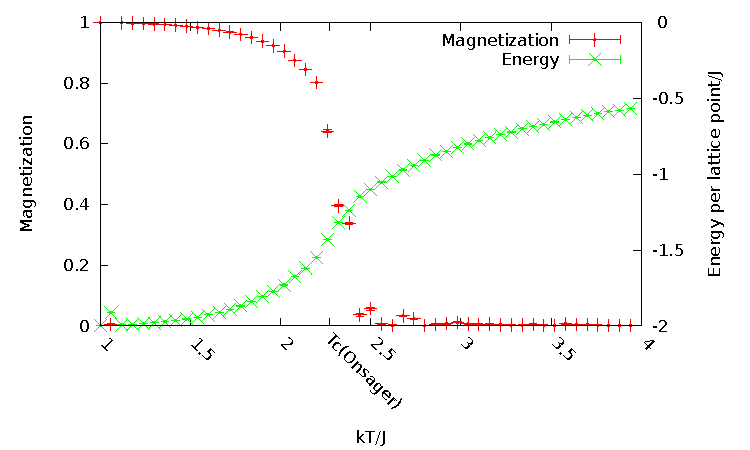
\includegraphics[width=\textwidth]{Optimized/tests/ising.pdf}
\caption{Energy and Magnetisation at varying temperature. It can be seen a phase transition occurs around Onsager's predicted critical temperature.}\label{fig:ising}
\end{figure}

\Fref{fig:ising} shows the simulation clearly demonstrates the predicted phase transition from a magnetised low energy phase at temperatures below \unit[$T\approx2.5$]{$J/k_B$} to a non-magnetic high energy phase at higher temperatures.

\begin{figure}
\center
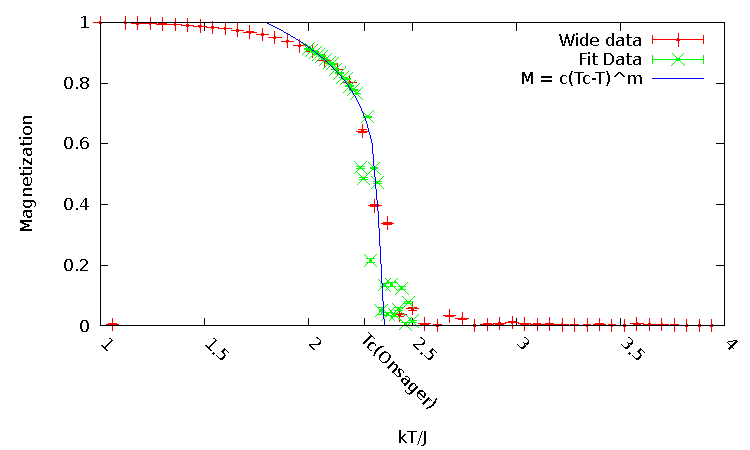
\includegraphics[width=\textwidth]{Optimized/tests/detail.pdf}
\caption{Magnetisation at varying temperature with a fit to the predicted behaviour just below the critical temperature. The fit gives \unit[$T_c=2.333\pm0.003$]{$J/k_B$} and $\beta=0.14\pm0.04$.}\label{fig:detail}
\end{figure}

\Fref{fig:detail} shows a fit\footnote{All fits made using the non-linear least squares implementation in Gnuplot.  This iterates the Marquardt-Levenberg algorithm adjusting parameters until the sum of the squares of the difference between the model and data is minimised. This algorithm gives an estimate in the fit parameters, shown in the graphs.} of data around the critical temperature to the $\left( T_c - T\right)^\beta$ prediction.  This gives \unit[$T_c=2.333\pm0.003$]{$J/k_B$} and $\beta=0.14\pm0.04$.  The $T_c$ calculated is 3\% away from Onsager's theoretical result---reasonable but less accurate than the error suggests.

\begin{figure}
\center
\includegraphics[width=\textwidth]{Optimized/tests/gridsize.pdf}
\caption{Calculated $T_c$ as a function of the size of grid. A linear fit suggests with infinite grid \unit[$T_c=2.296\pm0.009$]{$J/k_B$}}\label{fig:gridsize}
\end{figure}

To test if the error is caused by our simulating using a finite grid, \fref{fig:gridsize} shows the calculated $T_c$ as the grid size  was varied to see if the limit for large grid sizes tended towards the Onsager solution.  Extrapolating to an infinite grid (linear fit to $1/\textrm{number of lattice points}$) gives \unit[$T_c=2.296\pm0.009$]{$J/k_B$}, which is still 1.1\% out, far beyond the fit uncertainty.  This may be caused by having under-estimated the errors, or further difference between the simulation and theoretical model.

\begin{figure}
\center
\includegraphics[width=\textwidth]{Optimized/tests/heat.pdf}
\caption{Energy and the specific heat capacity estimates at varying temperature. Note the maximum heat capacity is around $T_c$.}\label{fig:heat}
\end{figure}



\section{Conclusions}
\label{sec:conclusions}

\bibliography{../../refs.bib}
\bibliographystyle{unsrt}

\appendix

\section{Source Code}
\label{sec:source-code}

Following are files of code written for this project. Required also is the source from the gnuplot iostream interface \cite{gnuplot-iostream}.  The project is designed for use with a build infrastructure part of the submitted package, it can be build minimally with:
\lstset{
language=sh,
basicstyle=\small\tt,
tabsize=4,
title=\lstname,
breaklines=true,
frame=single,
breakatwhitespace=true,
keywordstyle=\color[rgb]{0,0,1},
commentstyle=\color[rgb]{0.133,0.545,0.133},
stringstyle=\color[rgb]{0.627,0.126,0.941},
xleftmargin=-5.75em,
xrightmargin=-5.75em
}
\begin{lstlisting}
g++ -O2 -o ising ising.cc lattice.cc ../gnuplot-iostream/gnuplot-iostream.cc -DOUTPUT_GNUPLOT -DDEFAULT_J=1 -DDEFAULT_muH=0 -DDEFAULT_kT=1 -DDEFAULT_SIZE=20 -DPACKAGE=\"ising\" -lboost_iostreams -lutil
g++ -O2 -o runs runs.cc ../gnuplot-iostream/gnuplot-iostream.cc -DOUTPUT_GNUPLOT -DDEFAULT_J=1 -DDEFAULT_muH=0 -DDEFAULT_kT=1 -DDEFAULT_SIZE=20 -DPACKAGE=\"ising\" -lboost_iostreams -lutil
\end{lstlisting}

\lstset{language=C++}
\lstinputlisting{src/ising.cc}
\lstinputlisting{src/lattice.h}
\lstinputlisting{src/lattice.cc}
\lstinputlisting{src/runs.cc}
\end{document}